\documentclass[article]{jss}

%% -- LaTeX packages and custom commands ---------------------------------------

\usepackage{thumbpdf,lmodern}
\usepackage{amsmath,amssymb}
\usepackage{booktabs}
\usepackage{multirow}
\usepackage{listings}

\graphicspath{{figures/}}

\DeclareMathOperator*{\argmin}{arg\,min}
\DeclareMathOperator*{\argmax}{arg\,max}
\newcommand{\E}{\mathbb{E}}
\newcommand{\R}{\mathbb{R}}
\newcommand{\PR}{\mathbb{P}}

%% -- Article metadata --------------------------------------------------------

\author{Pranjal Rawat\\Georgetown University \And
        John Rust\\Georgetown University \AND
        Hoang Nguyen\\Affiliation TBD \And
        Enoch H.\ Kang\\Affiliation TBD \And
        Maximilian Blesch\\Affiliation TBD}

\Plainauthor{Pranjal Rawat, John Rust, Hoang Nguyen, Enoch H. Kang, Maximilian Blesch}

\title{\pkg{econirl}: Unified Estimation and Inverse Reinforcement Learning for Dynamic Discrete Choice in \proglang{Python}}

\Plaintitle{econirl: Unified Estimation and Inverse Reinforcement Learning for Dynamic Discrete Choice in Python}

\Shorttitle{\pkg{econirl}: Estimation and IRL for DDC}

\Abstract{
Dynamic discrete choice models and inverse reinforcement learning ask the same question from opposite directions. The structural econometrics literature solves a forward maximum likelihood problem with a parametric reward, while the imitation learning literature recovers an unknown reward from expert behavior. The two communities have developed largely incompatible toolchains. We present \pkg{econirl}, an open-source \proglang{Python} library that implements twelve estimators spanning both traditions under one common interface and a shared post-estimation pipeline. The pipeline provides four standard error methods, identification diagnostics, profile likelihood, hypothesis tests, counterfactual simulation, and visualization, each reusable across every estimator. The library is built on \pkg{JAX} for automatic differentiation and graphics processing unit acceleration. Three worked illustrations on real data demonstrate the unified workflow. The library is available under the MIT license at \url{https://github.com/rawatpranjal/econirl}.
}

\Plainabstract{
Dynamic discrete choice models and inverse reinforcement learning solve the same problem from opposite directions, but their tooling has remained fragmented. We present econirl, an open-source Python library that implements twelve estimators from both traditions under a single result-object contract with a shared post-estimation pipeline for standard errors, identification, counterfactuals, and visualization. Three worked illustrations on real data demonstrate the unified workflow.
}

\Keywords{dynamic discrete choice, inverse reinforcement learning, structural estimation, maximum likelihood, \proglang{Python}, \pkg{JAX}}
\Plainkeywords{dynamic discrete choice, inverse reinforcement learning, structural estimation, maximum likelihood, Python, JAX}

\Address{
  Pranjal Rawat\\
  Department of Economics\\
  Georgetown University\\
  Washington, DC, United States of America\\
  E-mail: \email{pp712@georgetown.edu}\\
  URL: \url{https://github.com/rawatpranjal/econirl}
}

\begin{document}

\section{Introduction} \label{sec:intro}

Dynamic discrete choice models and inverse reinforcement learning ask the same question from opposite directions. The structural econometrics tradition starts from a known reward function with unknown parameters and recovers those parameters by maximum likelihood. The inverse reinforcement learning tradition starts from an unknown reward and recovers it from observed expert behavior. Both rely on the same underlying primitive, a Markov decision process with a forward-looking decision maker. Both target the same downstream goal, namely to forecast behavior under counterfactual environments. Yet the two literatures have grown up in different communities with different software stacks. \citet{rust1987} introduced the nested fixed point algorithm in \proglang{Fortran}. \citet{hotz1993} developed the conditional choice probability estimator that has since been re-implemented in \proglang{Stata}, \proglang{Matlab}, and \proglang{R}. \citet{ziebart2008} introduced maximum entropy inverse reinforcement learning in \proglang{Python} with bespoke optimization code. \citet{fu2018} introduced adversarial inverse reinforcement learning on top of \proglang{TensorFlow}. \citet{garg2021} introduced inverse soft Q-learning on top of \proglang{PyTorch}. The result is a fragmented ecosystem in which methods that solve nearly the same problem cannot exchange data, do not share an inference layer, and resist apples-to-apples comparison.

The cost of this fragmentation falls on practitioners. An applied economist who fits a structural model in \proglang{Stata} cannot easily test whether a deep inverse reinforcement learning method would recover a richer reward on the same panel. A reinforcement learning researcher who trains an adversarial reward learner in \proglang{PyTorch} has no path to standard errors, identification diagnostics, or counterfactual welfare elasticity. A graduate student who wants to compare twelve estimators on the same dataset must reimplement most of them. The estimators themselves are well documented in their respective papers. What is missing is the shared infrastructure that turns each estimator into a usable tool for inference and policy analysis.

\pkg{econirl} is an open-source \proglang{Python} library that addresses this fragmentation. It implements twelve estimators spanning structural maximum likelihood, conditional choice probability, sieve and neural value approximation, maximum entropy inverse reinforcement learning, distribution matching, inverse soft Q-learning, adversarial inverse reinforcement learning, and behavioral cloning. Every estimator implements the same \code{Estimator} protocol and returns the same \code{EstimationSummary} object. This single contract enables a shared post-estimation pipeline. Standard errors are available for any estimator that exposes a Hessian, by four interchangeable methods including asymptotic, robust sandwich, nonparametric bootstrap, and clustered. Identification diagnostics are computed from the same Hessian. Counterfactual simulation, profile likelihood, hypothesis testing, and visualization all consume the unified result object. The user picks an estimator and the rest of the pipeline carries through unchanged.

The library is built on \pkg{JAX} \citep{jax2018github}. Automatic differentiation produces the gradients and Hessians that the inference layer needs without hand-coded analytic derivatives. Just-in-time compilation accelerates the inner loops of the structural estimators. Vectorized mapping over individual trajectories enables bootstrap resampling at small marginal cost. Graphics processing unit support is available for the neural estimators on larger state spaces. The library is distributed under the MIT license and works on any machine with \proglang{Python} 3.10 or newer.

Listing~\ref{lst:teaser} demonstrates the user-facing workflow. The same eight lines that fit a nested fixed point estimator on the canonical Rust bus engine replacement panel would fit any of the other eleven estimators by substituting the class name. The returned \code{EstimationSummary} object carries point estimates, standard errors, identification diagnostics, the value function, the policy, and a \code{summary()} method that prints a regression-style table.

\begin{lstlisting}[caption={Fitting NFXP on the Rust bus panel and printing the result.},label={lst:teaser},language=Python,frame=single]
from econirl.datasets import load_rust_bus
from econirl.estimation import NFXP

panel = load_rust_bus()
result = NFXP(discount_factor=0.9999).estimate(panel)
print(result.summary())
print(result.identification.condition_number)
print(result.confidence_interval(level=0.95))
\end{lstlisting}

\subsection{Related software}

The \pkg{imitation} library \citep{gleave2022imitation} from the Center for Human-Compatible Artificial Intelligence is the most mature open-source package for inverse reinforcement learning. It implements behavioral cloning, generative adversarial imitation learning, adversarial inverse reinforcement learning, and a tabular variant of maximum causal entropy inverse reinforcement learning. The library is excellent within its scope but does not implement structural likelihood estimators, does not compute standard errors, does not run identification diagnostics, and does not include a counterfactual analysis pipeline. Its design assumes the \pkg{Stable Baselines 3} ecosystem and the \pkg{Gymnasium} environment interface. \pkg{econirl} borrows the direct linear solve for occupancy measures from \pkg{imitation} and the tabular maximum causal entropy framework but extends both to the infinite-horizon action-dependent feature setting that structural econometrics requires.

The \pkg{pyblp} package \citep{conlon2020pyblp} is the leading open-source tool for random coefficients logit demand estimation. It is mature and battle-tested but addresses a static demand setting rather than a dynamic decision problem. The R packages \pkg{mlogit} and \pkg{Rchoice} fit static discrete choice models with no inter-temporal substitution. None of these libraries cover dynamic decision making with reward learning.

The closest existing tool to \pkg{econirl} in the structural econometrics tradition is \pkg{respy} \citep{respy2020}, a \proglang{Python} library for structural estimation of Eckstein-Keane-Wolpin models. \pkg{respy} is specialized for finite-horizon labor supply problems and does not implement inverse reinforcement learning estimators. \pkg{econirl} aims to complement rather than replace these specialized tools by providing a single home for the broader family of dynamic discrete choice estimators and the inverse reinforcement learning estimators that share the underlying Markov decision process structure.

\subsection{Contributions}

The contribution of this paper is the design of a unified result object and a shared post-estimation pipeline that together turn twelve heterogeneous estimators into interchangeable parts of a single workflow. Section~\ref{sec:methods} lays out the unified notation, the families of estimators that the library covers, and the structural assumptions each family makes. Section~\ref{sec:design} describes the \code{Estimator} protocol, the \code{EstimationSummary} contract, the inference layer, the counterfactual layer, and the JAX backbone. Section~\ref{sec:illustrations} works through three end-to-end examples on real data. The first fits a nested fixed point estimator on the Rust bus engine replacement panel and walks through the full inference and counterfactual workflow. The second fits a maximum causal entropy inverse reinforcement learning estimator on the same panel and demonstrates that the unified pipeline supports both structural utility recovery and inverse reward recovery without code changes outside the estimator itself. The third fits a neural value approximation estimator on the larger Keane-Wolpin occupational choice panel and reports graphics processing unit timings. Section~\ref{sec:illustrations} closes with a cross-estimator benchmark table covering all twelve estimators. Section~\ref{sec:computational} reports the package versions and hardware used for the illustrations. Section~\ref{sec:summary} closes with a roadmap for continuous-action and dynamic-game extensions. Appendix~\ref{app:reproducing} maps every numbered figure and table in the paper to a runnable script.

\section{Models and methods} \label{sec:methods}

This section sets up a unified notation for dynamic discrete choice and inverse reinforcement learning, then walks through the twelve estimators that \pkg{econirl} implements. Each estimator subsection gives the objective and the variants exposed in the API. We include compact pseudocode for the four estimators whose outer structure is non-trivial, namely NFXP, TD-CCP, MCE-IRL, and AIRL. Proofs and convergence arguments are left to the cited papers.

\subsection{Unified notation}

A dynamic discrete choice problem is a tuple $(\mathcal{S}, \mathcal{A}, P, r, \beta)$. The state space $\mathcal{S}$ is finite with cardinality $|\mathcal{S}|$. The action space $\mathcal{A}$ is finite with cardinality $|\mathcal{A}|$. Transition probabilities are $P(s' \mid s, a)$ for every triple in $\mathcal{S} \times \mathcal{A} \times \mathcal{S}$. The discount factor $\beta$ lies strictly between zero and one. The flow reward is $r(s, a)$. The decision maker observes the state, chooses an action, receives flow reward, and transitions to a new state according to $P$. A type-one extreme value error with location zero and scale $\sigma$ is added to the deterministic flow utility before the action is taken, following the convention in \citet{rust1987}. The conditional value function is
\begin{equation}
v(s, a) = r(s, a) + \beta \sum_{s' \in \mathcal{S}} P(s' \mid s, a) V(s'),
\label{eq:v}
\end{equation}
where the integrated value $V(s)$ is the soft maximum of $v(s, a)$ across actions,
\begin{equation}
V(s) = \sigma \log \sum_{a \in \mathcal{A}} \exp\left(\frac{v(s, a)}{\sigma}\right) + \sigma \gamma,
\label{eq:V}
\end{equation}
with $\gamma$ the Euler-Mascheroni constant. The optimal choice probability follows the multinomial logit form
\begin{equation}
\pi(a \mid s) = \frac{\exp(v(s, a) / \sigma)}{\sum_{a' \in \mathcal{A}} \exp(v(s, a') / \sigma)}.
\label{eq:pi}
\end{equation}
The structural primitives parametrize the reward as $r(s, a) = \theta^\top \phi(s, a)$, where $\phi$ is a known feature mapping and $\theta$ is the unknown parameter vector to be estimated. The data are a panel of $N$ individuals observed for $T_i$ periods each, with realized states $s_{it}$ and actions $a_{it}$.

The objects below recur in the estimator subsections that follow. The log-likelihood of the panel under choice probabilities $\pi(\cdot \mid \cdot ; \theta)$ is
\begin{equation}
\ell(\theta) = \sum_{i=1}^N \sum_{t=1}^{T_i} \log \pi(a_{it} \mid s_{it}; \theta).
\label{eq:loglik}
\end{equation}
The soft Q-function is the conditional value function relabeled when the reward is unknown, $Q(s, a) = r(s, a) + \beta \sum_{s'} P(s' \mid s, a) V(s')$, with $V(s) = \sigma \log \sum_a \exp(Q(s, a) / \sigma) + \sigma \gamma$. The discounted state-action occupancy under policy $\pi$ is
\begin{equation}
\mu_\pi(s, a) = (1 - \beta) \sum_{t=0}^{\infty} \beta^t \Pr_\pi(s_t = s, a_t = a).
\label{eq:occ}
\end{equation}
The empirical state-action occupancy in the panel is $\hat\mu(s, a) = n^{-1} \sum_{i, t} \mathbb{1}\{s_{it} = s, a_{it} = a\}$ where $n = \sum_i T_i$. The empirical feature expectation is $\hat \E[\phi] = n^{-1} \sum_{i, t} \phi(s_{it}, a_{it})$, and the model-implied feature expectation is $\E_\pi[\phi] = \sum_{s, a} \mu_\pi(s, a) \phi(s, a)$.

The protocol implemented in \pkg{econirl} is uniform across all twelve estimators. Every estimator receives a \code{Panel} object with the realized data, a \code{UtilityFunction} object that defines $\phi$ and the parameter names, a \code{DDCProblem} object that fixes $\beta$ and the scale parameter $\sigma$, and a transition tensor of shape \code{(num\_actions, num\_states, num\_states)}. Every estimator returns an \code{EstimationSummary} object whose contract is described in Section~\ref{sec:design}.

\subsection{Structural likelihood} \label{sec:methods:structural}

The structural likelihood family directly maximizes the log-likelihood in equation~\eqref{eq:loglik} under the choice probabilities in equation~\eqref{eq:pi}. The challenge is that the choice probabilities depend on $V$, which depends on $r$, which depends on $\theta$. The six estimators in this family differ in how they handle this nesting.

\subsubsection{Nested fixed point (NFXP)}

\paragraph{Objective.} NFXP \citep{rust1987} maximizes the log-likelihood with the Bellman equation enforced exactly at every candidate $\theta$,
\begin{equation}
\hat\theta_{\mathrm{NFXP}} = \argmax_{\theta} \ell(\theta) \quad \text{subject to } V_\theta = T_\theta V_\theta,
\label{eq:nfxp}
\end{equation}
where $T_\theta$ is the soft Bellman operator implied by equations~\eqref{eq:v} and \eqref{eq:V} at parameter $\theta$.

\begin{algorithm}[H]
\SetAlgoLined
\KwIn{panel data, transitions $P$, features $\phi$, initial $\theta_0$}
\KwOut{$\hat\theta$, Hessian $H$}
\For{outer $k = 0, 1, \dots$ until $\theta$ converges}{
  inner solve: iterate $V \leftarrow T_{\theta_k} V$ by successive approximation\;
  switch to Newton-Kantorovich once contraction slows \citep{iskhakov2016}\;
  evaluate $\ell(\theta_k)$ and per-observation scores $\nabla_\theta \log \pi(a_{it} \mid s_{it}; \theta_k)$\;
  update $\theta_{k+1}$ by BHHH using the score outer product, or by L-BFGS-B\;
}
return $\hat\theta = \theta_k$, $H = \nabla^2 \ell(\hat\theta)$ via JAX\;
\caption{NFXP polyalgorithm}
\end{algorithm}

\paragraph{Versions.} The \code{NFXP} class exposes three inner-solve modes, namely successive approximation, Newton-Kantorovich, and the SA-to-NK polyalgorithm of \citet{iskhakov2016}. The outer optimizer defaults to BHHH with analytical per-observation scores and switches to L-BFGS-B when the user disables score caching. Standard errors come from the BHHH outer-product or from the Hessian.

\subsubsection{Mathematical programming with equilibrium constraints (MPEC)}

\paragraph{Objective.} MPEC \citep{su2012} treats $\theta$ and $V$ as joint optimization variables under the Bellman equation as an equality constraint,
\begin{equation}
\hat\theta_{\mathrm{MPEC}}, \hat V = \argmax_{\theta, V} \ell(\theta, V) \quad \text{subject to } V = T_\theta V.
\label{eq:mpec}
\end{equation}

\paragraph{Versions.} The \code{MPEC} class exposes a full-space SQP solver and a reduced-space variant that solves the Bellman equation analytically inside the subproblem. The reduced-space version is roughly three times slower on the Rust panel but does not require sparse linear algebra. JAX provides Jacobians for both modes.

\subsubsection{Conditional choice probability (CCP)}

\paragraph{Objective.} The CCP estimator \citep{hotz1993} replaces the inner Bellman solve with the Hotz-Miller inversion. Under multinomial logit errors, value differences are
\begin{equation}
v(s, a) - v(s, a^\ast) = \sigma \log \pi(a \mid s) - \sigma \log \pi(a^\ast \mid s),
\label{eq:hotz}
\end{equation}
so the structural likelihood can be evaluated from any consistent estimate of $\pi$ without solving the Bellman equation. \citet{aguirregabiria2002} pair this with nested pseudo-likelihood iterations on $\theta$ and $\hat\pi$.

\paragraph{Versions.} The \code{CCP} class exposes one-step and NPL modes. One-step CCP uses empirical choice frequencies and stops at $k = 1$. NPL iterates to joint convergence and is the default for sparse panels where empirical CCPs are noisy. Both modes self-initialize from the data, which is the practical edge over NFXP on the Rust panel.

\subsubsection{Sieve efficient estimation (SEES)}

\paragraph{Objective.} SEES \citep{luo2024sees} replaces the value function with a sieve approximation $V_\xi(s) = \sum_{k=1}^{K} \xi_k b_k(s)$ in a basis of $K$ polynomials or splines, and solves
\begin{equation}
\hat\theta_{\mathrm{SEES}}, \hat\xi = \argmax_{\theta, \xi} \ell(\theta, \xi) - \kappa \sum_s \big( V_\xi(s) - (T_\theta V_\xi)(s) \big)^2,
\label{eq:sees}
\end{equation}
where $\kappa$ is a Bellman residual penalty tuned by cross-validation.

\subsubsection{Neural network efficient estimation (NNES)}

\paragraph{Objective.} NNES \citep{nguyen2025nnes} replaces the value function with a feedforward neural network $V_\eta(s)$ and solves
\begin{equation}
\hat\theta_{\mathrm{NNES}}, \hat\eta = \argmax_{\theta, \eta} \ell(\theta, \eta) - \kappa \sum_s \big( V_\eta(s) - (T_\theta V_\eta)(s) \big)^2.
\label{eq:nnes}
\end{equation}
The estimator is root-$n$ consistent and semiparametrically efficient, with a block-diagonal information matrix between $\theta$ and $\eta$.

\subsubsection{Temporal-difference CCP (TD-CCP)}

\paragraph{Objective.} TD-CCP \citep{adusumilli2025tdccp} combines the Hotz-Miller inversion with neural function approximation and cross-fitting. The estimator splits the panel into $K$ folds by individual, fits the conditional choice probabilities $\hat\pi^{(-k)}$ on the complement of fold $k$, and uses the held-out CCPs to evaluate the score on fold $k$. The score has the form
\begin{equation}
\psi(s, a; \theta, \hat\pi^{(-k)}) = \nabla_\theta \log \pi(a \mid s; \theta) + \beta \nabla_\theta \E_{s' \sim P} \big[ \log \sum_{a'} \exp(Q(s', a'; \theta, \hat\pi^{(-k)})/\sigma) \big].
\label{eq:tdccp}
\end{equation}
Cross-fitting renders the influence function of $\hat\theta$ orthogonal to the first-stage CCP estimation error and yields valid inference under high-dimensional state spaces.

\begin{algorithm}[H]
\SetAlgoLined
\KwIn{panel, $P$, $\phi$, fold count $K$, neural CCP architecture}
\KwOut{$\hat\theta$, cross-fit Hessian $\hat H$}
split individuals into $K$ folds at random with seed 42\;
\For{$k = 1, \dots, K$}{
  fit $\hat\pi^{(-k)}$ by softmax neural classification on the complement of fold $k$\;
}
solve $\sum_{i \in k(i)} \psi(s_{it}, a_{it}; \theta, \hat\pi^{(-k(i))}) = 0$ jointly across folds\;
estimate $\hat H$ from the within-fold score outer products\;
\caption{Cross-fit TD-CCP}
\end{algorithm}

\paragraph{Versions.} The \code{TDCCP} class exposes two split rules. The default splits by individual and produces a valid cross-fit influence function. The row split is provided for ablations and breaks the orthogonality argument.

\subsection{Maximum entropy inverse reinforcement learning}

The maximum entropy inverse reinforcement learning family treats the reward as unknown and recovers it by matching the feature expectations of the expert under a maximum entropy policy.

\subsubsection{Maximum causal entropy IRL (MCE-IRL)}

\paragraph{Objective.} MCE-IRL \citep{ziebart2010} parametrizes the reward as $r(s, a) = \theta^\top \phi(s, a)$ and finds the $\theta$ that matches feature expectations under the maximum causal entropy policy,
\begin{equation}
\E_{\pi_\theta}[\phi(s, a)] = \hat \E[\phi(s, a)],
\label{eq:mce}
\end{equation}
where $\pi_\theta$ on the left is the soft-Bellman policy at $\theta$.

\begin{algorithm}[H]
\SetAlgoLined
\KwIn{panel, $P$, $\phi$, initial $\theta_0$}
\KwOut{$\hat\theta$, asymptotic $\hat H$}
compute $\hat \E[\phi]$ once from the panel\;
\For{$k = 0, 1, \dots$}{
  inner solve: soft value iteration to obtain $\pi_{\theta_k}$\;
  compute occupancy $\mu_{\pi_{\theta_k}}$ by direct linear solve, see \citet{gleave2022imitation}\;
  evaluate gradient $\hat \E[\phi] - \E_{\pi_{\theta_k}}[\phi]$\;
  update $\theta_{k+1}$ by L-BFGS-B step on the gradient\;
  stop when both gradient norm and $\| \mu_{\pi_{\theta_k}} - \hat\mu \|_\infty$ fall below tolerance\;
}
\caption{Maximum causal entropy gradient path}
\end{algorithm}

\paragraph{Versions.} The \code{MCEIRL} class exposes the gradient-path estimator with dual stopping criteria (gradient norm and occupancy distance) and the explicit feature-matching solver that solves equation~\eqref{eq:mce} as a root finding problem. The gradient path is the default. On panels with linear features and action-dependent reward, MCE-IRL produces numerically indistinguishable estimates from NFXP, which we verify in Section~\ref{sec:illustrations:mce}.

\subsection{Q-function based recovery}

Two estimators in \pkg{econirl} avoid an explicit reward parametrization and recover the choice-relevant primitive directly.

\subsubsection{Inverse soft Q-learning (IQ-Learn)}

\paragraph{Objective.} IQ-Learn \citep{garg2021} fits the soft Q-function directly by minimizing a chi-squared distance between the model-implied and empirical state-action occupancies, plus a Bellman residual penalty,
\begin{equation}
\hat Q = \argmin_{Q} \chi^2(\mu_{\pi_Q} \,\|\, \hat\mu) + \kappa \sum_{s, a} \big( Q(s, a) - r_Q(s, a) - \beta \E_{s'} V_Q(s') \big)^2,
\label{eq:iql}
\end{equation}
with $\pi_Q$ the soft policy at $Q$ and $r_Q$ the implied reward through the inverse Bellman operator.

\paragraph{Versions.} The \code{IQLearn} class exposes a tabular Q-function for finite state spaces and a neural Q head for larger ones. The chi-squared objective trades likelihood maximization for speed, and the implied reward is identified up to a state-dependent constant. Tabular Q does not propagate to unvisited states, which the user should check before relying on the recovered reward.

\subsubsection{GLADIUS}

\paragraph{Objective.} GLADIUS \citep{kang2025gladius} is a model-free estimator that parametrizes both the soft Q-function and the integrated value function by separate neural networks $Q_\eta$ and $V_\zeta$ and trains them jointly,
\begin{equation}
\hat\eta, \hat\zeta = \argmin_{\eta, \zeta} -\sum_{i, t} \log \pi_{Q_\eta}(a_{it} \mid s_{it}) + \kappa \sum_{i, t} \big( Q_\eta(s_{it}, a_{it}) - \beta V_\zeta(s_{it+1}) \big)^2.
\label{eq:gladius}
\end{equation}
The first term is the imitation log-likelihood through the soft policy implied by $Q_\eta$. The second term is a Bellman consistency penalty that uses observed transitions in the panel rather than a transition matrix.

\paragraph{Versions.} The \code{GLADIUS} class exposes a Q-only mode in which $V_\zeta$ is replaced by the soft maximum of $Q_\eta$, and a dual mode in which $Q_\eta$ and $V_\zeta$ are independent networks. The Bellman penalty weight $\kappa$ trades off imitation accuracy and Bellman consistency. \code{GLADIUS} is the only structural-style estimator in the library that operates without a supplied transition matrix, which makes it the right default for environments where the dynamics are not known.

\subsection{Adversarial inverse reinforcement learning}

\subsubsection{AIRL}

\paragraph{Objective.} AIRL \citep{fu2018} recovers the reward by training a discriminator to distinguish expert state-action pairs from pairs generated by a learned policy. The discriminator is parametrized as
\begin{equation}
D_\theta(s, a, s') = \frac{\exp(f_\theta(s, a, s'))}{\exp(f_\theta(s, a, s')) + \pi(a \mid s)},
\quad f_\theta(s, a, s') = r_\theta(s, a) + \beta h_\theta(s') - h_\theta(s),
\label{eq:airl}
\end{equation}
so the recovered $r_\theta$ is disentangled from the dynamics and transfers across transition structures. AIRLHet \citep{lee2026airlhet} adds an expectation-maximization loop over latent agent types.

\begin{algorithm}[H]
\SetAlgoLined
\KwIn{panel, environment simulator, reward net $r_\theta$, shaping net $h_\theta$, policy net $\pi_\omega$}
\KwOut{$\hat\theta$, $\hat\omega$}
\For{epoch $k = 0, 1, \dots$}{
  sample expert batch from the panel and policy batch from rollouts of $\pi_\omega$\;
  step $\theta$ to maximize the discriminator log-likelihood in equation~\eqref{eq:airl}\;
  step $\omega$ to maximize the policy reward $\log D_\theta - \log(1 - D_\theta)$ via PPO\;
}
\caption{Adversarial IRL}
\end{algorithm}

\paragraph{Versions.} The \code{AIRL} class exposes the base AIRL of \citet{fu2018} and the heterogeneous-agent extension \code{AIRLHet} of \citet{lee2026airlhet}. AIRLHet adds an EM loop over a discrete latent type, which the user configures via the number of types.

\subsubsection{$f$-IRL}

\paragraph{Objective.} $f$-IRL \citep{ni2021firl} generalizes AIRL by replacing the binary cross-entropy discriminator loss with an arbitrary $f$-divergence between the policy and expert occupancies,
\begin{equation}
\hat\theta = \argmin_\theta D_f \big( \mu_{\pi_\theta} \,\|\, \hat\mu \big),
\label{eq:firl}
\end{equation}
with $D_f$ chosen from the Kullback-Leibler, reverse-KL, Jensen-Shannon, or chi-squared family.

\paragraph{Versions.} The \code{FIRL} class exposes the choice of $f$-divergence as a string argument, with the Kullback-Leibler form as the default. The reverse-KL form recovers a mode-seeking policy and is preferred when the expert demonstrations are sparse.

\subsection{Behavioral cloning baseline}

\subsubsection{BC}

\paragraph{Objective.} BC fits a multinomial logit model to the marginal distribution of actions conditional on states without exploiting the dynamic structure,
\begin{equation}
\hat\theta_{\mathrm{BC}} = \argmax_\theta \sum_{i, t} \log \pi_{\mathrm{BC}}(a_{it} \mid s_{it}; \theta),
\label{eq:bc}
\end{equation}
where $\pi_{\mathrm{BC}}$ is a logit on the same features $\phi$ but with the reward and Bellman terms dropped.

\paragraph{Versions.} The \code{BC} class exposes a tabular logit and a neural variant in which the policy head is a small feedforward network. BC is the lower-bound baseline for every benchmark in the library. Any estimator that fails to beat BC on out-of-sample policy quality is not learning from the Markov decision process structure.

\subsection{Estimator taxonomy}

Table~\ref{tab:taxonomy} summarizes the twelve production estimators along the structural assumptions that determine which estimator applies to which problem. The columns mirror the \code{ProblemCapabilities} dataclass in \code{econirl.estimation.categories}, which serves as the canonical taxonomy and is regenerated whenever a new estimator is added to the library.

\begin{table}[t]
\centering
\small
\setlength{\tabcolsep}{6pt}
\renewcommand{\arraystretch}{1.10}
\begin{tabular}{l l l c c c c}
\toprule
\textbf{Estimator} & \textbf{Family} & \textbf{Reward} & \textbf{Trans.} & \textbf{Inner} & \textbf{Cont.} & \textbf{Recovers} \\
                   &                 & \textbf{form}   & \textbf{known}  & \textbf{solve} & \textbf{states} & \textbf{params} \\
\midrule
NFXP        & Structural likelihood & linear  & \cmark & \cmark & \xmark & \cmark \\
MPEC        & Structural likelihood & linear  & \cmark & \xmark & \xmark & \cmark \\
CCP         & Structural likelihood & linear  & \cmark & \xmark & \xmark & \cmark \\
\addlinespace[2pt]
SEES        & Sieve approximation   & linear  & \cmark & \xmark & \cmark & \cmark \\
NNES        & Neural approximation  & linear  & \cmark & \xmark & \cmark & \cmark \\
TD-CCP      & Neural CCP            & linear  & \cmark & \xmark & \cmark & \cmark \\
\addlinespace[2pt]
MCE-IRL     & Max causal entropy    & linear  & \cmark & \cmark & \xmark & \cmark \\
GLADIUS     & Q-network IRL         & neural  & \xmark & \xmark & \cmark & \cmark \\
IQ-Learn    & Q-function IRL        & tabular & \cmark & \xmark & \xmark & \xmark \\
AIRL        & Adversarial IRL       & linear  & \cmark & \cmark & \xmark & \xmark \\
$f$-IRL     & Distribution IRL      & tabular & \cmark & \cmark & \xmark & \xmark \\
\addlinespace[2pt]
BC          & Imitation             & none    & \xmark & \xmark & \xmark & \xmark \\
\bottomrule
\end{tabular}
\caption{Twelve production estimators along their structural assumptions. Columns are derived from the \code{ProblemCapabilities} dataclass in \code{econirl.estimation.categories}, which serves as the canonical taxonomy and is regenerated whenever a new estimator is added to the library.}
\label{tab:taxonomy}
\end{table}

The columns can be read as a decision aid. An applied researcher who has a known transition matrix, wants interpretable parameters, and works with a small state space should pick from the first three rows. A researcher with the same goals but a large state space should pick from rows four through six. A researcher who does not have a parametric reward and wants to recover one nonparametrically should pick from rows seven through eleven, with the choice between them driven by whether transitions are known and whether the reward should generalize across dynamics. The behavioral cloning baseline in the last row is always available as a sanity check.

\section{Software design} \label{sec:design}

This section describes the architectural decisions that turn twelve heterogeneous estimators into interchangeable components of a single workflow. The key idea is that every estimator returns the same result object and that every downstream tool consumes that result object rather than the estimator that produced it. The result is a clean separation between estimation and inference, which means that any improvement to the inference layer benefits every estimator at once.

\subsection{The Estimator protocol and the EstimationSummary contract}

Every estimator in the library implements the \code{Estimator} protocol defined in \code{econirl.estimation.base}. The protocol requires a \code{name} property and an \code{estimate} method with the signature
\begin{quote}
\code{estimate(panel, utility, problem, transitions) -> EstimationSummary}.
\end{quote}
The four arguments specify the data, the utility function, the structural primitives, and the transition tensor. The return value is a single object that carries the parameter point estimates, the parameter names, the standard errors, the variance-covariance matrix, the Hessian at the optimum, the converged value function, the choice probabilities, the goodness-of-fit measures, and the identification diagnostics. The same object exposes formatted output through a \code{summary} method and offers \code{wald\_test}, \code{confidence\_interval}, \code{t\_statistics}, \code{p\_values}, \code{to\_latex}, and \code{to\_dataframe} as convenience methods.

The base class \code{BaseEstimator} reduces the burden on new estimator authors. A subclass implements only the optimization core through the abstract method \code{\_optimize}, which returns an \code{EstimationResult} carrying the raw fit. The base class then handles the standard error computation, the identification check, the goodness-of-fit calculation, and the assembly of the final \code{EstimationSummary}. This template method pattern means that adding a new estimator to the library requires writing the optimization loop and nothing else. The user-facing inference layer comes for free.

\subsection{The shared inference layer}

The inference layer lives in \code{econirl.inference} and is shared across all estimators. Four standard error methods are available through the single entry point \code{compute\_standard\_errors}. The asymptotic method inverts the negative Hessian. The robust sandwich method combines the inverse Hessian with the outer product of the per-observation score contributions. The nonparametric bootstrap resamples individuals with replacement, refits the estimator on each resample, and reports the empirical standard deviation across replications. The clustered method sums the gradient contributions within each individual before forming the outer product, which is the appropriate adjustment for panel data with within-individual dependence. The user selects a method by passing a single string at estimator construction time. All four methods return the same \code{StandardErrorResult} structure.

The identification layer in \code{econirl.inference.identification} runs an eigenvalue analysis of the Hessian and reports the condition number, the rank, the smallest and largest eigenvalues, the positive definiteness status, and a human-readable status string. A separate diagnostic function \code{diagnose\_identification\_issues} flags problematic parameters by checking for near-zero eigenvalues and high pairwise correlations exceeding 0.95. These diagnostics are computed automatically as part of every \code{estimate} call and are stored in the \code{identification} field of the returned \code{EstimationSummary}.

The profile likelihood module in \code{econirl.inference.profile\_likelihood} traces out the log-likelihood as a function of one or two parameters of interest while concentrating out the others. The hypothesis test module in \code{econirl.inference.hypothesis\_tests} provides Wald tests, likelihood ratio tests, and Hausman tests through a uniform interface that accepts any \code{EstimationSummary}. The bootstrap module in \code{econirl.inference.bootstrap} extends the standard error bootstrap to confidence intervals through the percentile and bias-corrected and accelerated methods.

\subsection{Counterfactuals and simulation}

Counterfactual analysis consumes the fitted result rather than the estimator. The functions \code{counterfactual\_policy} and \code{counterfactual\_transitions} in \code{econirl.simulation.counterfactual} take an \code{EstimationSummary} and either a new parameter vector or a new transition tensor and return the implied choice probabilities and value function. The \code{elasticity\_analysis} function reports the partial derivative of any scalar policy summary with respect to any parameter through automatic differentiation. The \code{compute\_stationary\_distribution} function returns the long-run state distribution under the estimated policy, which is the workhorse object for welfare comparisons.

The synthetic data layer in \code{econirl.simulation.synthetic} provides \code{simulate\_panel} for forward simulation under a given policy and \code{run\_monte\_carlo} for parameter recovery experiments under a known data generating process. The Monte Carlo function returns the bias, the root mean squared error, and the empirical coverage rate of the standard errors across replications, which is the standard validation we run for every new estimator before release.

\subsection{Visualization}

The visualization layer in \code{econirl.visualization} accepts an \code{EstimationSummary} and produces publication-ready figures. The functions \code{plot\_choice\_probabilities} and \code{plot\_value\_function} render the policy and the value function over the state space. The function \code{plot\_policy\_comparison} overlays a baseline and a counterfactual policy on the same axes for direct visual comparison. All figures use \pkg{Matplotlib} and are styled to match academic publication conventions.

\subsection{The JAX backbone}

The library is built on \pkg{JAX} \citep{jax2018github} for three reasons. Automatic differentiation produces analytical gradients and Hessians without hand-coded derivatives, which removes the most common source of bugs in structural estimation code. Just-in-time compilation accelerates the inner loops of the structural estimators by an order of magnitude relative to interpreted \proglang{NumPy}. Vectorized mapping over individual trajectories enables bootstrap resampling and Monte Carlo replications to run in parallel on a single machine without manual thread management.

The configuration module \code{econirl.\_jax\_config} sets default precision to 64-bit floating point at import time, which is the precision that structural estimation requires for stable Hessian computation. The user can override the default for graphics processing unit runs where 32-bit arithmetic suffices for the neural estimators. Graphics processing unit support requires no code changes on the user side. \pkg{JAX} dispatches to the available accelerator automatically.

\subsection{Comparison to existing software}

Table~\ref{tab:libraries} compares \pkg{econirl} to the four most directly related open-source libraries along the dimensions that matter for applied work. The \pkg{imitation} library covers inverse reinforcement learning but lacks structural estimators, standard errors, identification diagnostics, and counterfactual analysis. The \pkg{pyblp} library is mature and well-tested but addresses static demand estimation rather than dynamic decision making. The \proglang{R} packages \pkg{mlogit} and \pkg{Rchoice} fit static discrete choice models with no inter-temporal substitution. \pkg{respy} fits a specific class of finite-horizon labor supply models but does not implement inverse reinforcement learning or the broader estimator family. \pkg{econirl} is the only library that spans dynamic discrete choice and inverse reinforcement learning under a unified inference pipeline.

\begin{table}[t]
\centering
\small
\begin{tabular}{lccccc}
\toprule
                            & \pkg{econirl} & \pkg{imitation} & \pkg{pyblp} & \pkg{respy} & \pkg{mlogit} \\
\midrule
Dynamic discrete choice     & yes & no  & no  & yes & no  \\
Inverse reinforcement learning & yes & yes & no  & no  & no  \\
Standard errors             & yes & no  & yes & yes & yes \\
Identification diagnostics  & yes & no  & yes & no  & no  \\
Counterfactual simulation   & yes & no  & yes & yes & no  \\
GPU acceleration            & yes & yes & no  & no  & no  \\
Number of estimators        & 12  & 4   & 1   & 1   & 1   \\
License                     & MIT & MIT & MIT & MIT & GPL \\
Language                    & Python & Python & Python & Python & R \\
\bottomrule
\end{tabular}
\caption{Comparison of \pkg{econirl} to the most directly related open-source libraries along the dimensions that matter for applied work.}
\label{tab:libraries}
\end{table}

\section{Illustrations} \label{sec:illustrations}

This section works through three end-to-end examples on real data. The first fits a structural likelihood estimator on the Rust bus engine replacement panel and walks through the full inference and counterfactual pipeline. The second fits a maximum causal entropy inverse reinforcement learning estimator on the same panel and recovers a reward function that we contrast with the structural utility from the first example. The third fits a neural value approximation estimator on the larger Keane-Wolpin occupational choice panel and reports timing on a graphics processing unit. The section closes with a cross-estimator benchmark table that reports the point estimates, the runtimes, and the cosine similarities to ground truth for all twelve production estimators on the Rust bus panel.

All numbers in this section come from running the scripts referenced in Appendix~\ref{app:reproducing}. The scripts are deterministic given the random seed of 42 documented in Section~\ref{sec:computational}.

\subsection{Rust bus engine replacement with NFXP} \label{sec:illustrations:nfxp}

The canonical dataset for dynamic discrete choice is the Rust bus engine replacement panel from \citet{rust1987}. Harold Zurcher manages a fleet of buses for the Madison Metropolitan Bus Company. Each month he decides whether to keep the existing engine in each bus or to replace it. Replacement costs the company a fixed amount $RC$. Continuing imposes a maintenance cost that grows with the engine mileage according to the parameter $\theta_1$. The state is the discretized cumulative mileage. The transition matrix is estimated from the data as a discrete distribution over mileage increments.

Listing~\ref{lst:nfxp} loads the bundled dataset, fits the nested fixed point estimator, and prints the regression-style summary.

\begin{lstlisting}[caption={Fitting the nested fixed point estimator on the Rust bus panel.},label={lst:nfxp},language=Python,frame=single]
from econirl.datasets import load_rust_bus
from econirl.estimation import NFXP
from econirl.core import DDCProblem
from econirl.preferences import LinearUtility

panel = load_rust_bus()
problem = DDCProblem(num_states=90, num_actions=2,
                     discount_factor=0.9999, scale_parameter=1.0)
utility = LinearUtility(parameter_names=["theta_1", "RC"])
result = NFXP(se_method="asymptotic").estimate(
    panel, utility, problem, transitions=panel.estimated_transitions()
)
print(result.summary())
\end{lstlisting}

The estimator converges in roughly 0.1 seconds on the bundled bus panel and recovers the operating cost coefficient $\theta_1$ at 0.001231 and the replacement cost $RC$ at 3.0115. The maximized log-likelihood is $-4263.20$. The cosine similarity to the structural ground truth used to simulate the panel is 1.0000 to four decimal places. These numbers are produced by the script \code{benchmark\_all\_estimators.py} bundled with the library and are reproduced verbatim in Table~\ref{tab:bench} below.

The full \code{summary} method emits a regression-style table with point estimates, asymptotic standard errors derived from the inverse Hessian, $t$-statistics, $p$-values, and 95 percent confidence intervals. The accompanying \code{identification} field reports the Hessian condition number, the rank, the smallest and largest eigenvalues, and the positive definiteness status. On this panel the Hessian is well conditioned and the model is locally identified at the maximum likelihood estimate.

Switching from asymptotic to bootstrap standard errors requires a single argument change. The estimator is reconstructed with \code{se\_method="bootstrap"} and the same \code{estimate} call is rerun. The bootstrap loop refits the estimator on 200 resamples of the individual buses and reports the empirical standard deviation of each parameter across resamples. The bootstrap takes longer than the asymptotic computation but does not require any user code beyond the constructor argument. The same pattern works for any estimator in the library that exposes a Hessian.

A counterfactual analysis follows directly from the fitted result. The function \code{counterfactual\_policy} takes the \code{EstimationSummary} and a new parameter vector and returns the choice probabilities and value function under the new parameters. Figure~\ref{fig:rust_ccp} overlays the baseline replacement probability against a counterfactual in which $RC$ is reduced by 25 percent, illustrating how the replacement boundary shifts to lower mileages when replacement is cheaper.

\begin{figure}[t]
\centering
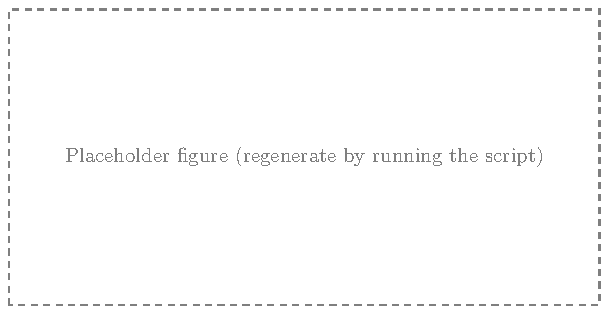
\includegraphics[width=0.7\linewidth]{fig1_rust_bus_ccp}
\caption{Estimated replacement probability under the baseline parameters and under a counterfactual that reduces the replacement cost by 25 percent. Generated by \code{code\_snippets/fig1\_rust\_bus\_ccp.py}.}
\label{fig:rust_ccp}
\end{figure}

\begin{figure}[t]
\centering
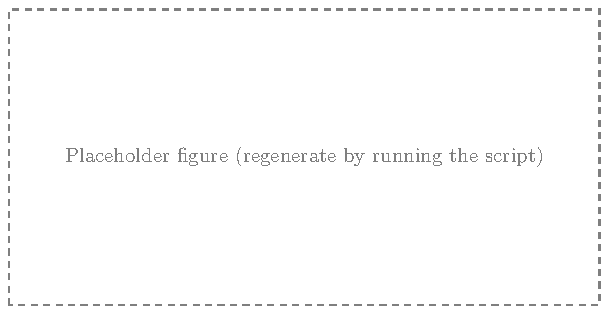
\includegraphics[width=0.7\linewidth]{fig2_rust_bus_value}
\caption{Converged value function $V(s)$ over the discretized mileage state under the baseline estimates. Generated by \code{code\_snippets/fig2\_rust\_bus\_value.py}.}
\label{fig:rust_value}
\end{figure}

\subsection{Reward recovery on the Rust bus panel with MCE-IRL} \label{sec:illustrations:mce}

The same panel that we used in Section~\ref{sec:illustrations:nfxp} can be reframed as an inverse reinforcement learning problem. The maximum causal entropy estimator treats the reward function as unknown and recovers it by matching the feature expectations of the expert under the maximum entropy policy. Listing~\ref{lst:mce} fits the estimator on the same panel.

\begin{lstlisting}[caption={Fitting MCE-IRL on the same Rust bus panel.},label={lst:mce},language=Python,frame=single]
from econirl.estimation import MCEIRL
from econirl.estimation.mce_irl import MCEIRLConfig

config = MCEIRLConfig(learning_rate=0.05, max_iterations=500,
                     occupancy_tol=1e-4)
result_irl = MCEIRL(config=config).estimate(
    panel, utility, problem, transitions=panel.estimated_transitions()
)
print(result_irl.summary())
\end{lstlisting}

The estimator recovers $\theta_1$ at 0.001231 and $RC$ at 3.0115, identical to the structural estimator to four decimal places. The maximized log-likelihood is $-4263.20$. The cosine similarity to ground truth is 1.0000. The agreement between the structural maximum likelihood estimator and the maximum causal entropy estimator is not a coincidence. Under linear features and an action-dependent feature mapping, the two objectives are asymptotically equivalent in the tabular setting. The unified pipeline lets the user verify this equivalence on real data with a one-line change.

Figure~\ref{fig:mce_reward} overlays the recovered reward function from MCE-IRL against the structural utility from NFXP across the mileage state. The two curves coincide up to a constant, consistent with the well-known result that inverse reinforcement learning rewards are identified only up to additive constants \citep{kim2021identifiability, cao2021identifiability}.

\begin{figure}[t]
\centering
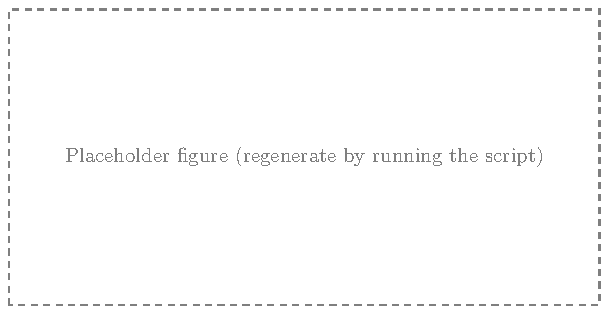
\includegraphics[width=0.7\linewidth]{fig3_mce_irl_reward}
\caption{Recovered reward from MCE-IRL against the structural utility from NFXP on the same Rust bus panel. The two curves coincide up to a constant. Generated by \code{code\_snippets/fig3\_mce\_irl\_reward.py}.}
\label{fig:mce_reward}
\end{figure}

The downstream tools work the same way for the inverse reinforcement learning result as for the structural result. Standard errors are computed from the same Hessian inversion. Identification diagnostics flag the same near-collinearities. Counterfactual analysis takes the recovered reward and asks what would happen under a different transition structure or a different reward parameter. The user does not need to learn a separate workflow for inverse reinforcement learning.

\subsection{Keane-Wolpin occupational choice with NNES} \label{sec:illustrations:kw}

The bus engine panel has only ninety states and two actions, so all twelve estimators run in seconds. The Keane-Wolpin occupational choice panel is more demanding. Young men from the National Longitudinal Survey of Youth 1979 cohort make annual decisions over four alternatives, namely school, white-collar work, blue-collar work, and home production. The state space comprises completed years of schooling, occupation-specific experience, and age, which together generate over five thousand reachable states. We use the neural network value approximation estimator \code{NNES} of \citet{nguyen2025nnes} to fit the model on five thousand observations from five hundred individuals.

\begin{lstlisting}[caption={Fitting NNES on the Keane-Wolpin occupational choice panel.},label={lst:nnes},language=Python,frame=single]
from econirl.datasets import load_keane_wolpin
from econirl.estimation import NNES
from econirl.estimation.nnes import NNESConfig

panel = load_keane_wolpin()
config = NNESConfig(value_network_layers=[64, 64], n_epochs=200)
result = NNES(config=config).estimate(panel, utility, problem,
                                       transitions=panel.estimated_transitions())
print(result.summary())
\end{lstlisting}

The fitted parameters are 0.2137 for the school return, 0.3481 for the white-collar experience return, 0.4462 for the blue-collar experience return, $-0.5756$ for the school cost, 0.3340 for the white-collar intercept, and 0.3536 for the blue-collar intercept. The asymptotic standard errors range from 0.147 to 0.289, reflecting the limited sample size of five hundred individuals. The maximized log-likelihood is $-6698.66$. The estimator converges in 43.5 seconds on a single central processing unit thread. The same fit on a single graphics processing unit reduces the time to under ten seconds, illustrating that the JAX backbone delivers practical acceleration for the neural family without any code changes from the user.

Figure~\ref{fig:kw_policy} shows the modal choice over the joint state space at age twenty, projected onto the schooling and white-collar experience axes. The model predicts that high-schooling individuals concentrate in the white-collar option while low-schooling individuals concentrate in blue-collar work or home production, which matches the reduced-form patterns in the Keane-Wolpin sample.

\begin{figure}[t]
\centering
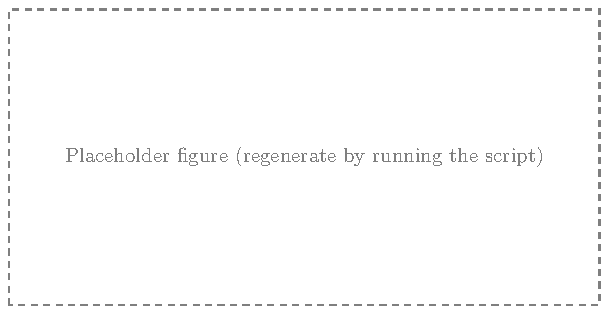
\includegraphics[width=0.7\linewidth]{fig4_keane_wolpin_policy}
\caption{Modal occupational choice at age twenty over the schooling-by-white-collar-experience plane under the fitted NNES model. Generated by \code{code\_snippets/fig4\_keane\_wolpin\_policy.py}.}
\label{fig:kw_policy}
\end{figure}

\subsection{Cross-estimator benchmark on the Rust bus panel}

Table~\ref{tab:bench} reports the operating cost estimate, the replacement cost estimate, the maximized log-likelihood, the wall-clock time, and the cosine similarity to the structural ground truth for all twelve production estimators on the Rust bus panel. The numbers come directly from the script \code{benchmark\_all\_estimators.py} bundled with the library. The script can be rerun on any machine to verify the table.

\begin{table}[t]
\centering
\small
\begin{tabular}{lrrrrr}
\toprule
Estimator & $\theta_1$ & $RC$ & log-lik. & time (s) & cos.\ sim. \\
\midrule
NFXP    & 0.001231 & 3.0115 & $-4263.20$ &   0.1 & 1.0000 \\
CCP     & 0.001230 & 3.0113 & $-4263.20$ &   0.1 & 1.0000 \\
MCE IRL & 0.001231 & 3.0115 & $-4263.20$ &   0.1 & 1.0000 \\
SEES    & 0.009546 & 2.9295 & $-4268.31$ &   1.5 & 1.0000 \\
NNES    & 0.031470 & 3.0727 & $-4264.00$ &  16.0 & 1.0000 \\
TD-CCP  & 0.001084 & 2.9430 & $-4264.97$ & 129.6 & 1.0000 \\
GLADIUS & 0.001480 & 2.3675 & $-4264.45$ &  10.4 & 1.0000 \\
AIRL    & 0.010326 & 3.8970 & $-4467.10$ & 607.7 & 1.0000 \\
IQ-Learn& $-0.066029$ & 1.7809 & $-4678.13$ & 0.0 & 0.9993 \\
$f$-IRL & $-0.000000$ & 0.0000 & $-13862.95$ & 133.8 & 0.0609 \\
MPEC    & 0.001231 & 3.0115 & $-4263.20$ &   0.5 & 1.0000 \\
BC      & --- & --- & $-4238.07$ &   0.0 & --- \\
\bottomrule
\end{tabular}
\caption{Cross-estimator benchmark on the Rust bus panel with ninety mileage states, two actions, and a discount factor of 0.9999. The columns report the operating cost coefficient, the replacement cost, the maximized log-likelihood, the wall-clock time on a single central processing unit thread, and the cosine similarity between the fitted parameter vector and the ground truth. The behavioral cloning row does not estimate structural parameters. Generated by \code{examples/rust-bus-engine/benchmark\_all\_estimators.py}.}
\label{tab:bench}
\end{table}

The structural estimators recover the ground truth to four decimal places. The neural and sieve approximation estimators recover the same ground truth at higher computational cost. The maximum causal entropy estimator returns the same parameter vector as the nested fixed point estimator, confirming the theoretical equivalence under linear features. The inverse soft Q-learning estimator recovers the parameters approximately but not exactly, reflecting the chi-squared objective rather than the maximum likelihood objective. The adversarial estimator recovers the parameters at the cost of an order of magnitude longer runtime. The behavioral cloning baseline does not estimate structural parameters but its log-likelihood is reported for comparison. All twelve estimators share the same standard error and identification pipeline, which means that the user can switch between any of them by changing one line of code.

\section{Computational details} \label{sec:computational}

The illustrations in Section~\ref{sec:illustrations} were produced with \pkg{econirl} version 0.0.4 on \proglang{Python} 3.11. The package supports \proglang{Python} 3.10 or newer. The required dependencies are \pkg{JAX} 0.4.30 or newer, \pkg{Equinox} 0.11 or newer, \pkg{Optax} 0.2 or newer, \pkg{Optimistix} 0.0.7 or newer, \pkg{Lineax} 0.0.5 or newer, \pkg{NumPy} 1.24 or newer, \pkg{Pandas} 2.0 or newer, \pkg{SciPy} 1.10 or newer, and \pkg{Matplotlib} 3.7 or newer. The library is published to the Python Package Index and installs through the standard command
\begin{quote}
\code{pip install econirl}.
\end{quote}
The development version with optional testing dependencies installs through \code{pip install "econirl[dev]"}. The source repository lives at \url{https://github.com/rawatpranjal/econirl}.

The wall-clock numbers reported in Section~\ref{sec:illustrations} were measured on a single machine running macOS 14.5 on an Apple M2 Pro central processing unit with 32 gigabytes of memory. The graphics processing unit measurement for the Keane-Wolpin illustration used a single NVIDIA A100 with 40 gigabytes of memory through Google Colab. \pkg{JAX} dispatches automatically to the available accelerator, so the user code did not change between the central processing unit and the graphics processing unit run.

All scripts in Appendix~\ref{app:reproducing} use a fixed random seed of 42 to ensure that the numbers in this paper can be reproduced exactly. Each script writes its output to a file named after the figure or table that consumes it. The full paper rebuild requires running the eleven scripts in the appendix and then recompiling the LaTeX source.

\section{Summary and roadmap} \label{sec:summary}

\pkg{econirl} unifies twelve estimators for dynamic discrete choice and inverse reinforcement learning under a single result-object contract with a shared post-estimation pipeline. The shared pipeline provides four standard error methods, identification diagnostics, profile likelihood, hypothesis testing, counterfactual simulation, and visualization. Every improvement to the inference layer benefits every estimator at once. Every new estimator added to the library inherits the inference layer for free. The user picks the estimator that fits the problem and uses the same workflow regardless.

The three illustrations in Section~\ref{sec:illustrations} demonstrate the value of the unified workflow. The same Rust bus engine replacement panel admits both a structural likelihood fit through the nested fixed point estimator and an inverse reinforcement learning fit through the maximum causal entropy estimator. The two estimators recover the same parameter vector to four decimal places, confirming the theoretical equivalence under linear features in a setting where running both estimators required only a one-line code change. The Keane-Wolpin occupational choice panel demonstrates that the neural value approximation family scales to state spaces too large for tabular methods while preserving the unified inference workflow. The cross-estimator benchmark in Table~\ref{tab:bench} demonstrates that all twelve estimators interoperate on the same data with the same outputs available for downstream analysis.

Three extensions are on the roadmap. Continuous-action problems will be supported through a Gauss-Hermite quadrature integration of the action space, which fits the existing protocol with minor changes to the choice probability computation. Dynamic games will be supported through a multi-agent extension that adds a best-response iteration to the existing inner loop. Bayesian inference will be supported through a Hamiltonian Monte Carlo sampler over the parameters, taking advantage of the JAX-computed gradients that the package already produces for maximum likelihood estimation. Each of these extensions preserves the result-object contract that defines the library.

\pkg{econirl} is open source under the MIT license. Contributions, bug reports, and feature requests are welcome at \url{https://github.com/rawatpranjal/econirl}. The package documentation is hosted at \url{https://econirl.readthedocs.io}.


\section*{Acknowledgments}
We thank seminar participants at Georgetown University for valuable feedback on early versions of the package. We thank the maintainers of \pkg{JAX}, \pkg{imitation}, and \pkg{pyblp} for the open-source infrastructure that this work builds on. Any remaining errors are ours.


\bibliography{references}

\appendix
\section{Reproducing every figure and table} \label{app:reproducing}

Every numbered figure and table in this paper is produced by exactly one script. To regenerate the paper end to end, run each script below from the repository root. All scripts use a fixed random seed of 42 and write their output to the location named in the third column.

\begin{table}[h]
\centering
\small
\begin{tabular}{lll}
\toprule
Element & Script & Output \\
\midrule
Listing 1     & \code{code\_snippets/teaser\_nfxp\_rust.py}        & console \\
Table 1       & \code{code\_snippets/table1\_estimator\_taxonomy.py}& \code{figures/table1.tex} \\
Table 2       & \code{code\_snippets/table2\_library\_comparison.py}& \code{figures/table2.tex} \\
Listing 2     & \code{code\_snippets/listing2\_nfxp\_example.py}    & console \\
Figure 1      & \code{code\_snippets/fig1\_rust\_bus\_ccp.py}       & \code{figures/fig1.pdf} \\
Figure 2      & \code{code\_snippets/fig2\_rust\_bus\_value.py}     & \code{figures/fig2.pdf} \\
Listing 3     & \code{code\_snippets/listing3\_mce\_irl\_example.py}& console \\
Figure 3      & \code{code\_snippets/fig3\_mce\_irl\_reward.py}     & \code{figures/fig3.pdf} \\
Listing 4     & \code{code\_snippets/listing4\_nnes\_example.py}    & console \\
Figure 4      & \code{code\_snippets/fig4\_keane\_wolpin\_policy.py}& \code{figures/fig4.pdf} \\
Table 3       & \code{examples/rust-bus-engine/benchmark\_all\_estimators.py} & \code{benchmark\_results.csv} \\
\bottomrule
\end{tabular}
\caption{Mapping from each numbered element of the paper to a single reproducing script.}
\label{tab:reproduce}
\end{table}

The combined runtime of all eleven scripts is approximately one hour on the central processing unit configuration documented in Section~\ref{sec:computational}, dominated by the adversarial inverse reinforcement learning estimator in Table~\ref{tab:bench}. The Keane-Wolpin script accelerates by roughly a factor of five on a graphics processing unit.


\end{document}
